\documentclass{article}
\usepackage{tikz}

\begin{document}

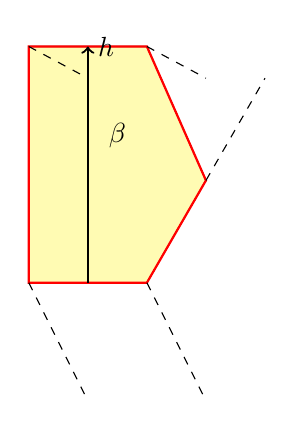
\begin{tikzpicture}[scale=1.5]
    % Draw the pentagonal base
    \draw[fill=yellow!30] (0,0) -- (1,0) -- (1.5,0.866) -- (1,2) -- (0,2) -- cycle;
    \draw[red, thick] (0,0) -- (1,0) -- (1.5,0.866) -- (1,2) -- (0,2) -- cycle;
    
    % Draw the height of the prism
    \draw[->, thick] (0.5,0) -- (0.5,2) node[right] {$h$};
    
    % Draw the dashed lines for the sides of the prism
    \draw[dashed] (0,0) -- (0.5,-1);
    \draw[dashed] (1,0) -- (1.5,-1);
    \draw[dashed] (1.5,0.866) -- (2,1.732);
    \draw[dashed] (1,2) -- (1.5,1.732);
    \draw[dashed] (0,2) -- (0.5,1.732);
    
    % Label the base
    \node at (0.75, 1.25) {\(\beta\)};
\end{tikzpicture}

\end{document}